\documentclass{article}
\usepackage[backend=biber,citestyle=ieee]{biblatex}
\usepackage[english]{babel}
% \usepackage[swedish]{babel}
\usepackage{graphicx}
\usepackage{csquotes}
\usepackage{float}
\usepackage{datetime}
\usepackage[title]{appendix}
\usepackage{subfig}
% \usepackage{a4wide} %For wider content on page
% \usepackage{amsmath} %For multiline equations 
\usepackage{fancyhdr}   %page header
\pagestyle{fancy}

% \usepackage[parfill]{parskip} %Line skip between paragraphs instead of indent

\usepackage{xcolor}
\usepackage{listings}

\definecolor{codegreen}{rgb}{0,0.6,0}
\definecolor{codegray}{rgb}{0.5,0.5,0.5}
\definecolor{codepurple}{rgb}{0.58,0,0.82}
\definecolor{backcolour}{rgb}{0.95,0.95,0.95}
\lstdefinestyle{mystyle}{
    backgroundcolor=\color{backcolour},   
    commentstyle=\color{codegreen},
    keywordstyle=\color{magenta},
    numberstyle=\tiny\color{codegray},
    stringstyle=\color{codepurple},
    basicstyle=\ttfamily\footnotesize,
    breakatwhitespace=false,         
    breaklines=true,                 
    captionpos=b,                    
    keepspaces=false,                 
    numbers=left,                    
    numbersep=5pt,                  
    showspaces=false,                
    showstringspaces=false,
    showtabs=false,                  
    tabsize=1
}
\lstset{style=mystyle}

\addbibresource{sources.bib}

\newcommand{\getauthor}{Elias Berglin} %Author
\newcommand{\gettitle}{Labb2} %Title

\newdateformat{daymonthyear}{\ordinal{DAY} \monthname[\THEMONTH] \THEYEAR} %Date

\title{\gettitle}
\author{\getauthor}

\date{\daymonthyear\today} %Remove for swedish date

\begin{document}

    % Title 
    \pagenumbering{gobble}
    \maketitle
    \newpage

    % Page header and footer
    \pagenumbering{arabic}
    \fancyhf{}
    \lhead{\getauthor}
    \rhead{\gettitle}
    \rfoot \thepage

    % Document starts here
    \section{Week 3}
    \subsection{Assignment}
    \subsubsection{Hough transform}
    The following graphs was created with the points given and with Hough transform applied:
    \begin{figure}[H]
        \centering
        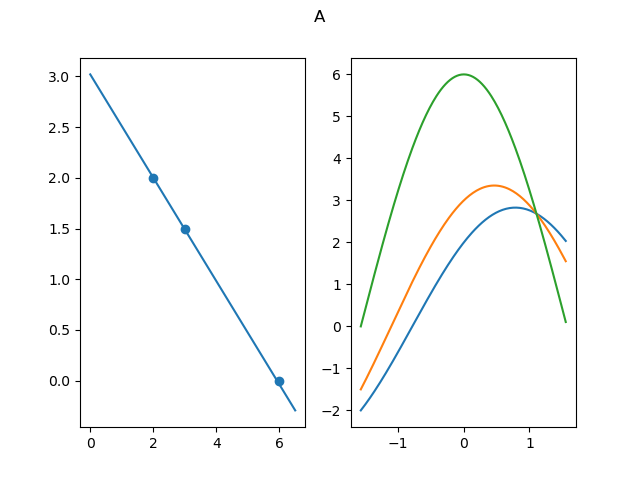
\includegraphics[width=1\textwidth]{Finished/HoughA.png}
    \end{figure}
    \begin{figure}[H]
        \centering
        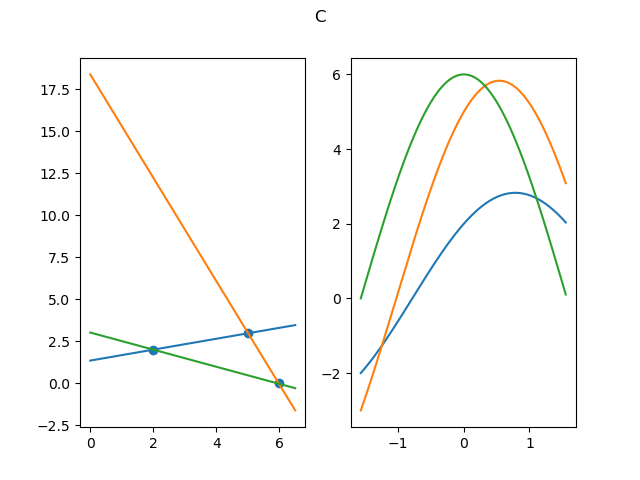
\includegraphics[width=1\textwidth]{Finished/HoughB.png}
    \end{figure}
    A quick note, Question b was not plotted due it being the same question as a
    \subsubsection{Feature descriptors}
    I have read 2 comparison papers between different feature descriptors. SIFT seems to always be the most acurate.
    But it is also not as fast. Considoring we have an AR application we need to have a somewhat faster algorithm
    to make it easier to track features. These papers say that ORB is almost as good as SIFT but much faster so I would
    go with ORB for my AR application. \cite{art1} \cite{tareen2018comparative}
    \subsubsection{Feature detection (and matching)}
    Python code used for the assignment can be found in appendix \ref{appendix:code}.
    Following images was generated:

    \begin{figure}[H]
        \centering
        \subfloat{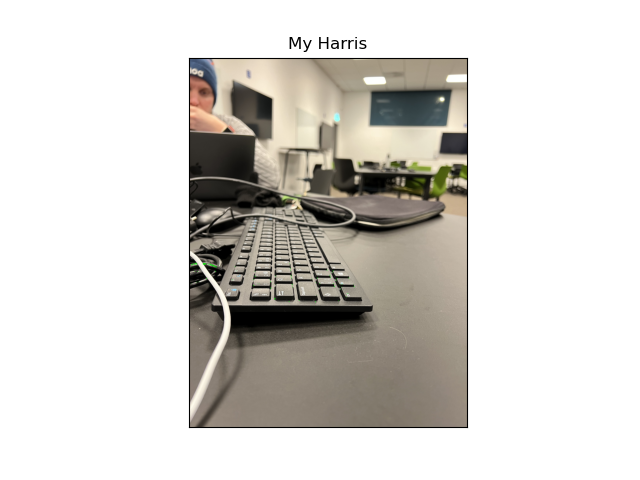
\includegraphics[width=8cm]{Finished/Start1_My_Harris_detector.png}}
        \quad
        \subfloat{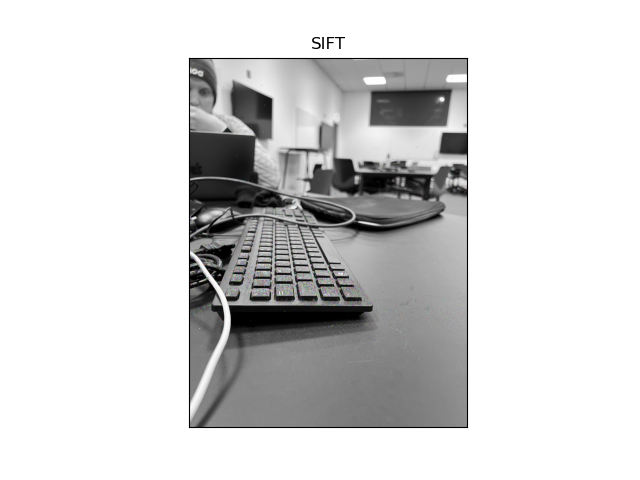
\includegraphics[width=8cm]{Finished/Start1_SIFT_Detector.png}}
        \caption{First image with Harris and SIFT}
    \end{figure}
    \begin{figure}[H]
        \centering
        \subfloat[]{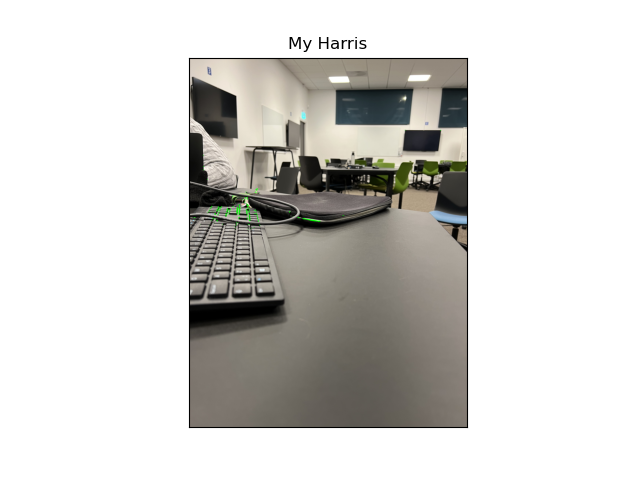
\includegraphics[width=8cm]{Finished/Start2_My_Harris_detector.png}}
        \quad
        \subfloat[]{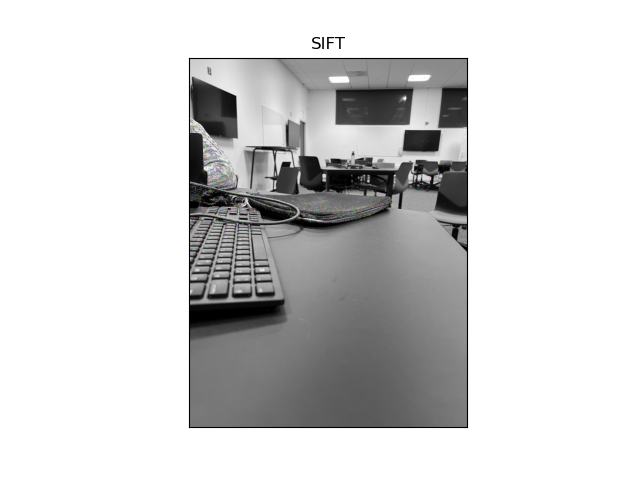
\includegraphics[width=8cm]{Finished/Start2_SIFT_Detector.png}}
        \caption{Second image with Harris and SIFT}
    \end{figure}
    \subsection{Reflection}
    This week was interesting. 
    I thought that feature detection/descriptors was a really interesting subject.
    The most interesting part was reading the research papers where they benchmarked
    different algorithms for finding features. I had a hard time grasping the concept
    of Hough transform but after watching the YouTube course I quickly understood
    how it worked. This has been the fact for all of the weeks. If I don't fully
    understand something during the lecture the YouTube course have always cleard
    it up for me.

    My Harris detector did not performe well compared to SIFT. But when I compared it
    to the OpenCV implementation it was not far off. From reading the papers \cite{art1} \cite{tareen2018comparative}
    I now understand that SIFT is really good at finding features and thus it is understandable that
    Harris does not perform ass well


    \section{Week 4}
    \subsection{Assingment}
    \subsubsection{2D Transformations}
    \subsubsection{Stereo estimation}
    \subsubsection{Plane Sweep}
    \subsubsection{Stitching}
    
    % Sources
    \newpage
    \printbibliography

    % Appendices
    \newpage
    \begin{appendices}

        \section{Code}
        \label{appendix:code}
        \begin{lstlisting}[language=Python]
            import cv2
import numpy as np
import matplotlib.pyplot as plt


def harris(img_name, window_size, k, threshold):
    img = cv2.imread(img_name)
    gray = cv2.cvtColor(img, cv2.COLOR_BGR2GRAY)
    img_gauss = cv2.GaussianBlur(gray, (3, 3), 0)
    h = img.shape[0]
    w = img.shape[1]

    matrix_r = np.zeros((h, w))

    dx = cv2.Sobel(img_gauss, cv2.CV_64F,1,0, ksize=3)
    dy = cv2.Sobel(img_gauss, cv2.CV_64F, 0, 1, ksize=3)

    dx2 = np.square(dx)
    dy2 = np.square(dy)
    dxy = dx * dy

    offset = int(window_size/2)
    print("Finding corners...")
    for y in range(offset, h-offset):
        for x in range(offset, w-offset):
            sx2 = np.sum(dx2[y-offset:y+1+offset, x-offset:x+1+offset])
            sy2 = np.sum(dy2[y-offset:y+1+offset, x-offset:x+1+offset])
            sxy = np.sum(dxy[y-offset:y+1+offset, x-offset:x+1+offset])

            H = np.array([[sx2, sxy], [sxy, sy2]])
            det = np.linalg.det(H)
            tr = np.matrix.trace(H)
            R = det - k * (tr ** 2)
            matrix_r[y - offset, x - offset] = R

    cv2.normalize(matrix_r, matrix_r, 0, 1, cv2.NORM_MINMAX)
    for y in range(offset, h - offset):
        for x in range(offset, w - offset):
            value = matrix_r[y, x]
            if value > threshold:
                cv2.circle(img, (x, y), 3, (0, 255, 0))

    plt.figure("Harris detector")
    plt.imshow(cv2.cvtColor(img, cv2.COLOR_BGR2RGB)), plt.title("My Harris")
    plt.xticks([]), plt.yticks([])
    plt.show()

def cv2Harris(img_name):
    img = cv2.imread(img_name)
    gray = cv2.cvtColor(img, cv2.COLOR_BGR2GRAY)

    harris = cv2.cornerHarris(gray, 2, 3, 0.04)
    harris = cv2.dilate(harris, None)
    img[harris > 0.01 * harris.max()] = [0, 0, 255]

    plt.figure("Harris detector")
    plt.imshow(cv2.cvtColor(img, cv2.COLOR_BGR2RGB)), plt.title("CV2 Harris")
    plt.xticks([]), plt.yticks([])
    plt.show()

def cv2Sift(img_name):
    img = cv2.imread(img_name)
    gray = cv2.cvtColor(img, cv2.COLOR_BGR2GRAY)
    sift = cv2.SIFT_create()
    kp = sift.detect(gray, None)

    img = cv2.drawKeypoints(gray, kp, img)
    plt.figure("SIFT Detector")
    plt.imshow(img), plt.title("SIFT")
    plt.xticks([]), plt.yticks([])
    plt.show()

img_name = "start2.jpeg"

harris(img_name, 5, 0.04, 0.30)
cv2Harris(img_name)
cv2Sift(img_name)

        \end{lstlisting}

    \end{appendices}

\end{document}

% list with a,b,c
% \begin{enumerate}[label=(\alph*)]
%     \item 
% \end{enumerate}

% Centered figure with caption:
% \begin{figure}[H]
%     \centering
%     \includegraphics[width=1\textwidth]{%path} 
%     \caption{}
%     \label{fig:}
% \end{figure}

% Side by side figures:
% \begin{figure}[H]
%     \centering
%     \subfloat{{\includegraphics[width=0.46\textwidth]{%path} }}%
%     \qquad
%     \subfloat{{\includegraphics[width=0.46\textwidth]{%path} }}%
%     \caption{}
%     \label{fig:}
% \end{figure}

% Table with caption:
% \begin{table}[H]      
%     \begin{center}
%     \begin{tabular}{|c|c|} 
%         \hline
%         \textbf{} & \textbf{} \\\hline\hline
%          &  \\\hline 
%     \end{tabular}
%     \end{center}
%     \caption{}
%     \label{tab:}
% \end{table}

% Equation on multiple lines
% \begin{equation}
%    \begin{split}
%        x &= y \\
%        y &= z
%    \end{split}
% \end{equation}

% Code snippet
% \begin{lstlisting}%[language=]
%    //Code here
% \end{lstlisting}

% Code snippet from source file 
% \lstinputlisting[language=]{%path}
